% (c) 2020 Stefan Antonowicz
% Based off of tex found at https://github.com/ludus-leonis/nipajin
% This file is released under Creative Commons Attribution-NonCommercial-ShareAlike 4.0 International License.
% Please do not apply other licenses one-way.

\renewcommand{\yggWonders}{%
  \mychapter{Wonders}{wonders}
}

\renewcommand{\yggWondersText}{%

%%%%%%%%%%%%%%%%%%%%%%%%%%%%%%%%%%%%%%%%%%%%
%%% STAFF MAGIC
%%%%%%%%%%%%%%%%%%%%%%%%%%%%%%%%%%%%%%%%%%%%


\mysection{Staff Magic}{wonder-staff-magic}

A staff can be a cane, club, wand, staff, caduceus, or walking stick; it is a necessary accessory for any Philosopher reaching the heights of their study. It must be made out of a special material: the more powerful the staff, the better the material must be.  If you're making an Iron level staff you might need a branch from an ash tree from the Forbidden Wood.  If you're making a Gold level staff, it might need to be the femur of the Great Wyrm Vermithrax.  Work this out with the Arbiter!

All staffs are 2-handed Fast Brawl weapons that do d6 damage.  They can produce light at will (as a Torch); can hit creatures only affected by magic weapons; and can dispel \mylink{Illusion}{wizardry-illusion} with a touch (though this will prompt a \mylink{Wizards' Duel}{philosopher-wizards-duel} if the opposing wizard is present).

If you do not wish anyone else to use this staff, it can be bound with a \mylink{Wizard Sigil}{research-sigil-wizard} created by you. As long as the staff has your Wizard Sigil on it, the staff is just a normal quarterstaff in anyone else's hands (though obviously made of special material!).

A Staff is limited to 3 powers, but you can "mix and match" from any group as you wish (so the staff could have 2 Iron powers and 1 Gold power if you wanted). These are just the most common abilities; you're encouraged to work out additional abilities with the Arbiter.

The "Stackable" column in the table indicates if the ability can be bought more than once.  When you see \NUM in a description, this is the number of times you bought the ability.

  \begin{center}
    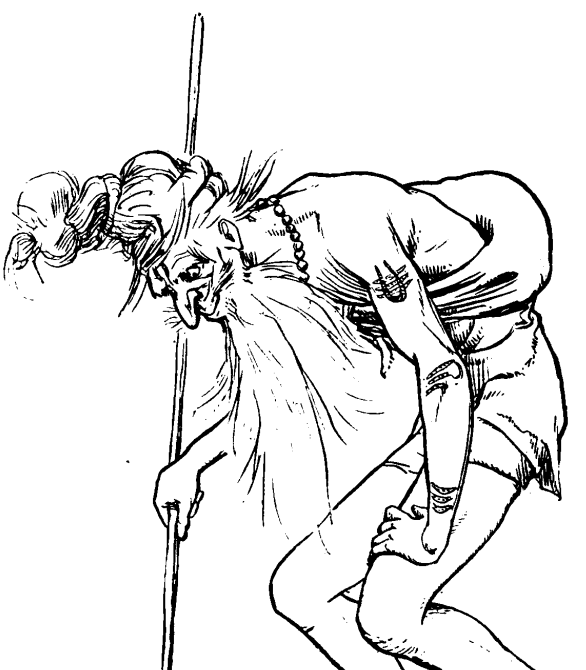
\includegraphics[scale=.5]{StaffMagic}
  \end{center}



\mysubsection{Iron Powers}{staff-magic-iron-powers}

    \example { 
        \COST  500\FE each
    }

  \mytable{X r}{
    \thead{Effect} & \thead{Stackable} \\
  }{
     All Saves +1 & No \\
     Anchor: d8 & No \\
     Blood: 1 & No \\
     Damage +1 & Yes \\    
     Daze & No \\
     Insight: +1 & Yes \\
     Mending & No \\
     Mitigation: Mishap to nothing & No \\
     Safe Casting & Yes \\
     Use your \INT for Fight Rolls\footnote{Instead of \VIG} & No \\
  }

\newpage


\mysubsection{Silver Powers}{staff-magic-silver-powers}
    \example { 
      \COST 1000\AG each
    }

  \mytable{X r}{
    \thead{Effect} & \thead{Stackable} \\
  }{
     All Saves +2 & No \\
     Anchor: d10 & No \\
     Blood: 2 & No \\
     Damage \DCUP & No \\
     Insight: +2 & Yes \\
     Mitigation: Calamity to Mishap & No \\
     Power Casting & Yes \\
     Rend & No \\
     Use your \INT for Fight\ and Guard\footnote{Instead of \DEX}  rolls & No \\
  }


\mysubsection{Gold Powers}{staff-magic-gold-powers}
\example { 
  \COST 2500\AU each
}

  \mytable{X r}{
    \thead{Effect} & \thead{Stackable} \\
  }{
     All Saves +4 & No \\
     Anchor: d12 & No \\
     Blood: 3 & No \\
     Cleave & No \\
     Damage \DCUP & Yes \\
     Insight: +3 & Yes \\
     Mitigation: Ruin to Calamity & No \\
     Natural Casting & Yes \\
     Wisdom & No \\
  }

\cbreak

\myhighlight{Anchor}{staff-magic-anchor}

Changes the die you roll with your \INT when rolling a Torrent, instead of a d6

\myhighlight{Blood}{staff-magic-blood}

Once per Session, you can tap into the power of the Staff directly and add 1 (Iron), 2 (Silver), or 3 (Gold) Blood Dice to your Pool.

\myhighlight{Insight}{staff-magic-insight}

Up to \NUM times a Session, you can add a +1,+2, or +3 (depending on the level) to any Knowledge roll.  You can only use this ability once per roll i.e.  you cannot use Insight: +2 twice on the same roll to get a +4

\myhighlight{Mending}{staff-magic-mending}

The \TARGET cost of \mylink{Mend}{leechcraft-mend} is 1 as long as the staff is in your possession.


\myhighlight{Mitigation}{staff-magic-mitigation}

Once per Session, Mitigation reduces the effect of a Ruin to a Calamity (Gold); a Calamity to a Mishap (Silver); and eliminates the effect of a Mishap (Iron).

\myhighlight{Natural Casting}{staff-magic-natural casting}

Your Blood Dice are only depleted on a natural 1 (instead of a 1 or 2). 


\myhighlight{Power Casting}{staff-magic-power casting}

You can replace one of your rolled Blood Die with a natural 6 (as if it was rolled) \NUM times per Session  

 

\myhighlight{Safe Casting}{staff-magic-safe casting}

You can replace one of your rolled Blood Die with a natural 1 (as if it was rolled) \NUM times per Session.

\myhighlight{Wisdom}{staff-magic-wisdom}

Whenever you fail a Leechcraft roll, the negative modifier is -1 instead of -2 (the modifiers are still cumulative).

\newpage



%%%%%%%%%%%%%%%%%%%%%%%%%%%%%%%%%%%%%%%%%%%%
%%% SWORD MAGIC
%%%%%%%%%%%%%%%%%%%%%%%%%%%%%%%%%%%%%%%%%%%%

\newpage

\mysection{Sword Magic}{spriggan-sword-magic}



\flavor{
  As the green flames, stung by her runes, leaped up, and the heat of the fire grew intenser, she stepped backwards further and further, and merely uttered her runes a little louder the further she got from the fire. She bade Alveric pile on logs, dark logs of oak that lay there cumbering the heath; and at once, as he dropped them on, the heat licked them up; and the witch went on pronouncing her louder runes, and the flames danced wild and green; and down in the embers the seventeen, whose paths had once crossed Earth's when they wandered free, knew heat again as great as they had known, even on that desperate ride that had brought them here. And when Alveric could no longer come near the fire, and the witch was some yards from it shouting her runes, the magical flames burned all the ashes away and that portent that flared on the hill as suddenly ceased, leaving only a circle that sullenly glowed on the ground, like the evil pool that glares where thermite has burst. And flat in the glow, all liquid still, lay the sword. \Tilde The King of Elfland's Daughter
}



The Rom who have turned their backs on Elfland still have some skill in writing the runes and glyphs of the Abandoned onto Mortal weapons: longswords, shortswords, daggers, and spears. 

\mysubsection{Magic Weapons}{spriggan-magic-weapons}

Enchanted weapons can all strike creatures that require magical weapons to hit, and can emit a small circle of bluish or greenish light at will (similar to the light cast by a few candles).

Weapons are often named after their wielder or maker, and the powers of the runes on the blade.  Some examples:

\mybullet {
  \item The Hallowed and Indestructible Spear of Yoon-Suin
  \item The Thrice Deadly Dagger of Kos
  \item The Flaming and Twice Accurate Sword of Magnuss
}


  \begin{center}
    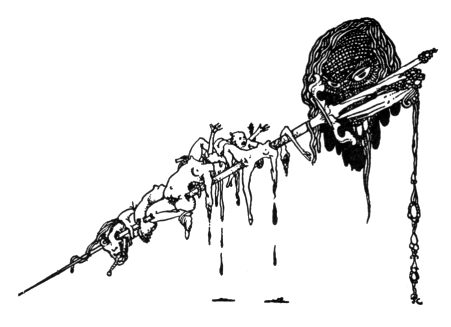
\includegraphics[scale=.5]{SwordMagic}
  \end{center}


\mysubsection{The Runes of Elfland}{spriggan-elfland-runes}

\mylist {

  \item You can place a maxiumum of 3 runes on a weapon

  \item Because Spriggan can't handle iron, the material of the weapon must be exotic (silver, gold, etc) or otherworldly (adamantium, meteorite).  The material needs to be available and should be worked out with the Arbiter.  Only daggers, swords (long and short), and spears can be enchanted

  \item In order to accept an enchantment, the weapon must have a Mortal sigil, mark, or writ etched onto the blade, once for each Elfland Rune.  Archaic runes require a \mylink{Wizard Sigil}{research-sigil-wizard}, Fiendish runes require a \mylink{Witch Mark}{occultism-witch-mark}, and Seraphic runes require a \mylink{Holy Writ}{miracle-holy-writ}.

  \item The weapons is enchanted with the help of the Abandoned.  You must summon one of the Abandoned for each rune you wish to etch on the blade; each Abandoned can write a single Elfland Rune on the weapon.  The Abandoned can only write in the language that they know:  Archons can only write Archaic Runes, Fiends can only write Fiendish Runes, and Seraphs can only write Seraphic Runes.

  \item  Aside from the cost of the weapon itself, you must pay for the materials necessary to perform the magic.  

  \mybullet{
    \item The first Rune costs 1,000\FE in materials.  
    \item The second Rune costs 2,500\AG in materials.  
    \item The third Rune cost 5,000\AU in materials.
  }


}
 
The runes on the next page will get you started.  Feel free to work with the Arbiter for additional powers.  

\newpage


\mysubsection{Archaic Runes}{spriggan-archaic-runes}

\mybold{ Cleaving}

The weapon has the Weapon Trait: Cleave

\mybold{ Dazing}

The weapon has the Weapon Trait: Daze

\mybold{ Hefty}

The weapon has the Weapon Trait: Hefty

\mybold{ Rending}

The weapon has the Weapon Trait: Rend

\mybold{ Brutal}

The weapon has the Weapon Trait: Brutal

\mybold{ Lucky}

The weapon has a d4 \UD that can be used to add to any \RO attempt you're making. You can use this \UD to add to any \RO attempt you're making (including Fight and Guard).  The \UD is restored at the start of the next Session.

\mysubsection{Fiendish Runes}{spriggan-fiendish-runes}


\mybold{ Accurate}


Adds +1 to your Fight \RO when using this weapon.  This Rune can be written more than once.

\mybold{ Shielding}


Add +1 to your Guard \RO when using this weapon.  This Rune can be written more than once

\mybold{ Deadly}


The weapon's damage is \DCUP.  This Rune can be written more than once.

\mybold{Flaming}


In addition to its normal damage, the weapon deals +d4 fire damage.  On a Crit, the victim must make a Save vs. Doom or be lit on fire for d4 Markovian (+d3 damage at the top of the Moment)

\mybold{Icy}


In addition to its normal damage, the weapon deals +d4 ice damage.  On a Crit, the victim must make a Save vs. Doom or be paralyzed for d4 Markovian.

\mybold{ Bloodletting}


In addition to its normal damage, the weapon inflicts Bleeding when it hits Flesh.


\mysubsection{Seraphic Runes}{spriggan-seraphic-runes}


\mybold{ Hallowed}


In addition to its normal damage, the weapon deals +d4 extra damage to the Unhallowed.  This Rune can be written more than once.

\mybold{ Indestructible}


The weapon cannot be destroyed by non-magical means (acid, rust, etc.), and it gets a +4 to its Saves against being destroyed by magical means (even if it would normally not get a Save).  The sword uses your Save vs Doom for its Saves.

\mybold{ Tenacious}

The weapon cannot be dropped unless wielder wills it.  If you are struck down, there is no way to remove the weapon from your hand short of cutting the hand off (which breaks the enchantment)


\mybold{ Infamous}

When you deal a killing blow with this weapon, the victim's \myital{noumenon} is briefly revealed (for most creatures, it appears as a small, vaporous homunculus which vanishes after a few moments).  This immediately forces a morale check for all enemies that are Close.

\mybold{ Vigilant}


When in your hands, you can see invisible creatures, and you have both Day Vision and Dark Vision (and you can switch between them at will).  You cannot be surprised while the weapon is in your hands.

\mybold{ Rallying}


When you deal a killing blow with this weapon, your allies automatically win Init in the next Moment.


}%end
